\chapter{Interactive Object Recognition}
\label{chapter:Object Recognition}

\section{Challenges}
As suggested in Chapter \ref{chapter:Introduction} in feature-matching-based object recognition systems we encounter a lot of difficulties that mainly stem from view-point-variance of the features as well as lighting conditions and noisy sensors. In order to prove that hypothesis, we implemented an object recognition system that extracts the features in the  live images and matches them against features extracted from the images in the database. Based on the number of matches the system can detect which object is seen in the live image.

\subsection{Lighting Conditions and Sensor Noise}

During our experiments we noticed that a lot of features in the live image were flickering even though we did not change position of any object in the image. After investigating this issue we came to the conclusion that the disability of the feature detector to find the same feature in two consecutive frames is mainly caused by sensor noise and changing lighting conditions. We examined that by searching for the features in the same image location and then matching them against the live image. We saved two patches: one depicting the feature found in the database image, and the second one showing the matched feature in the live image.

Figure \ref{fig:patches} shows two pairs of above described patches taken at two consecutive frames and the difference between them. Looking at the difference image (see last column in Figure \ref{fig:patches}) it can be clearly seen that there was a significant change in the live image even though we did not change anything in our set-up. Corner detector did not find the correct feature in the live image simply because this image looks differently which is caused by the sensor noise and the change of lighting conditions.

\begin{figure}
\centering

{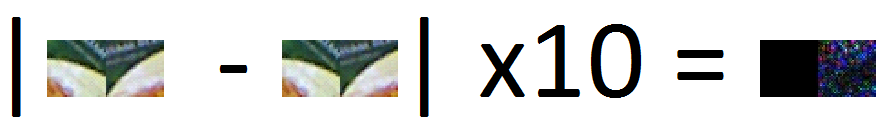
\includegraphics[width=1\columnwidth]{figures/patches.png}}

\caption{Difference between two pairs of images taken without taking any action to objects in between. The first patch of the pair shows the area in the database image where the feature was found. The second patch shows the area in the live image where the corresponding match was found. After subtracting one pair from another(second pair of patches was taken a at the same pixel location but the match was not found) and multiplying the difference by the factor of 10, the significant difference in live image patch is visible. There is no difference in the database image patch because it is the same patch for both pairs.  It indicates the influence that lighting and sensor noise have on the image. }
\label{fig:patches}
\end{figure}

\begin{figure}
\centering
    \begin{tabular}{c}
 

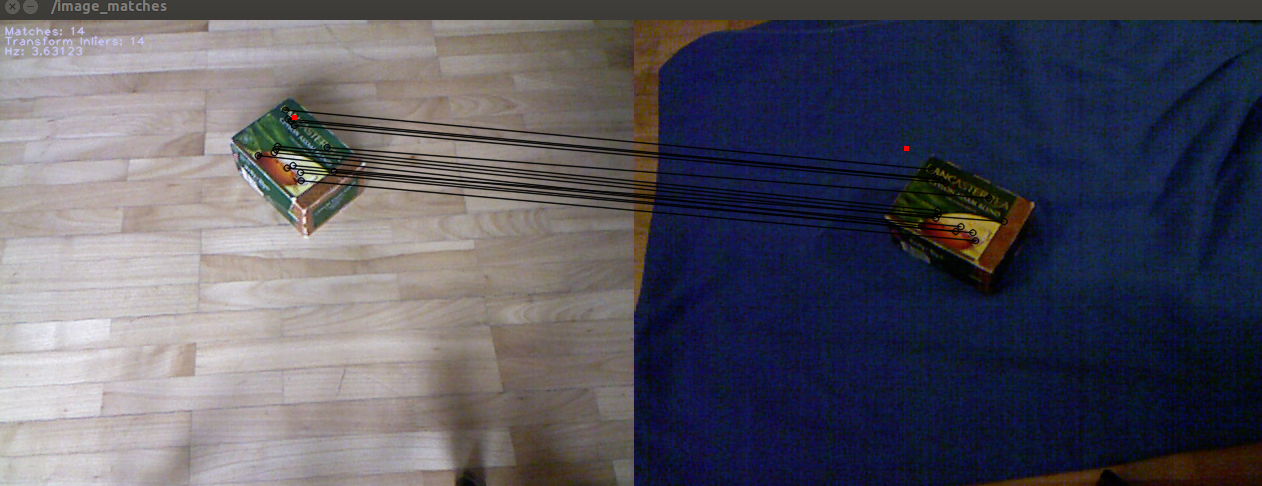
\includegraphics[width=0.7\columnwidth]{figures/sift-gpu-no-rotation.png}\\
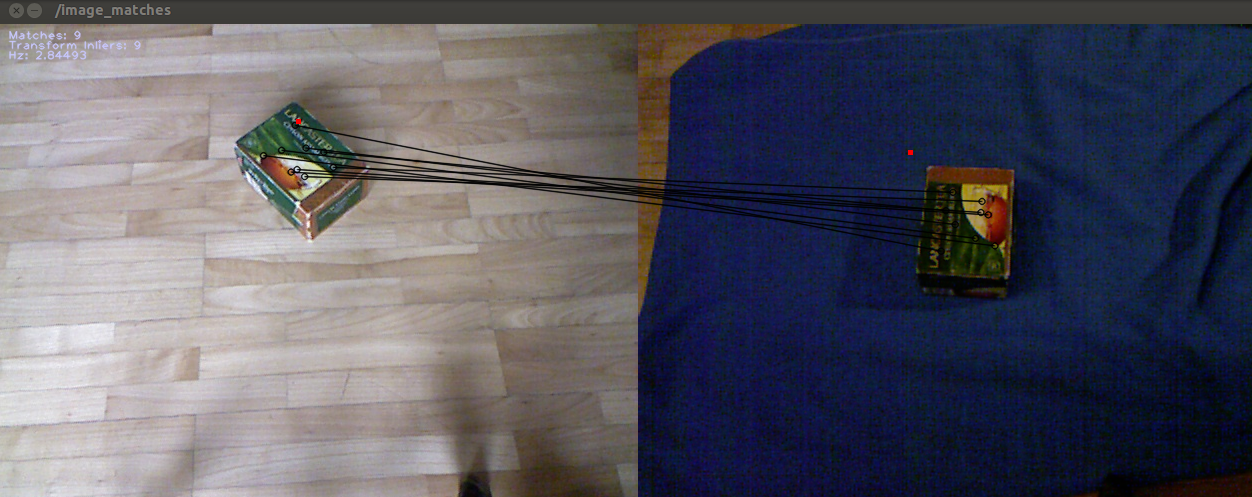
\includegraphics[width=0.7\columnwidth]{figures/siftgpu-rotation.png}\\
    \end{tabular}


\caption{Comparison of two pairs of images using SIFT detector and SIFT descriptor. The upper image shows the object in the original pose whereas the lower shows the rotated object. It can be noticed that number of feature matches significantly decreases if the object is rotated. }
\label{fig:sift-features}
\end{figure}

\begin{figure}
\centering
    \begin{tabular}{c}
 

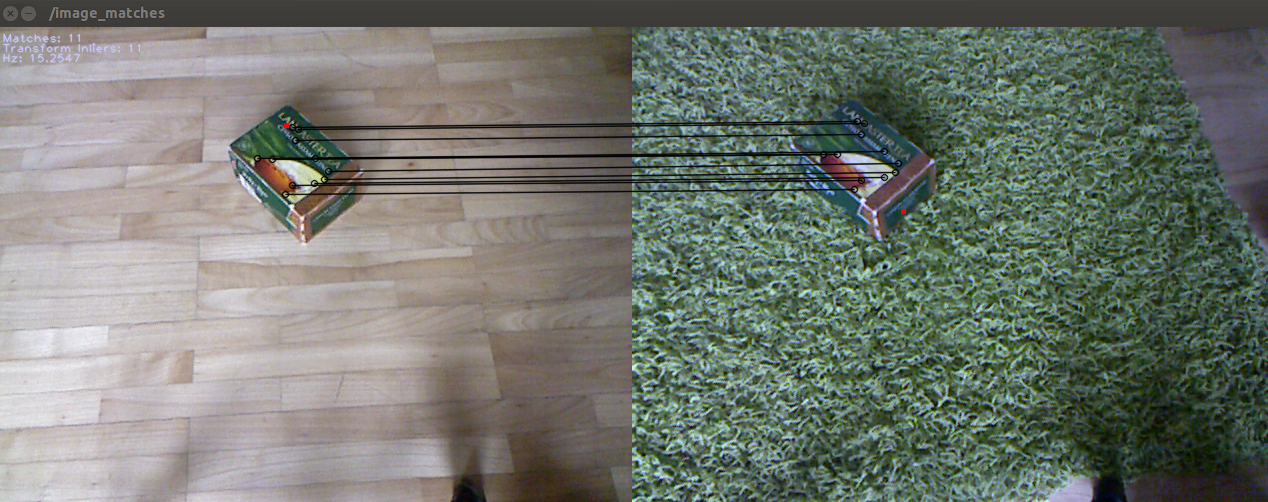
\includegraphics[width=0.7\columnwidth]{figures/freak-no-rotation.png}\\
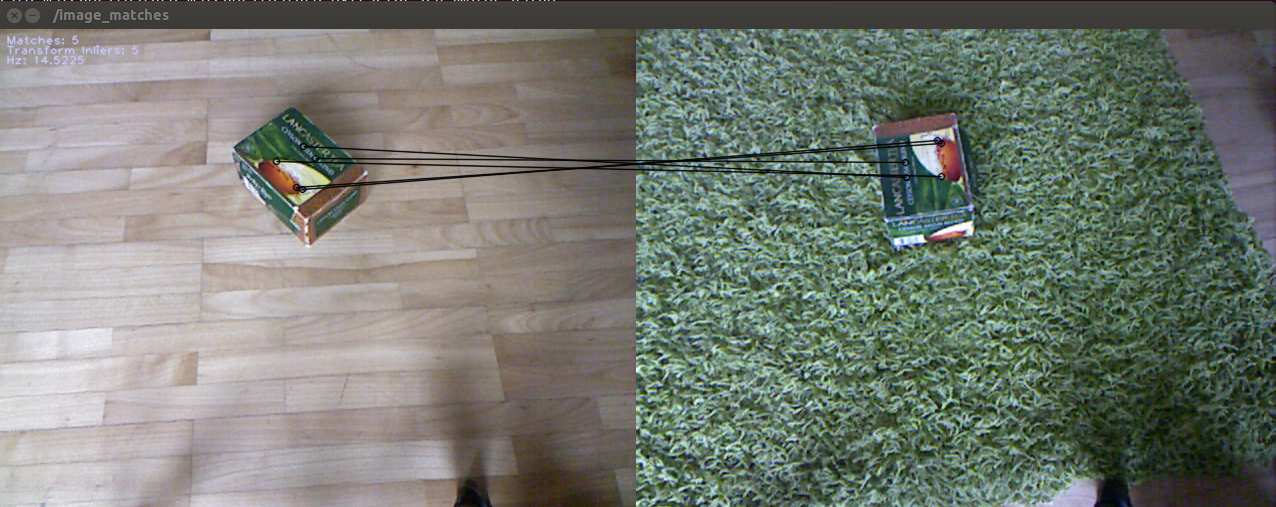
\includegraphics[width=0.7\columnwidth]{figures/freak-rotation.png}\\
    \end{tabular}


\caption{Comparison of two pairs of images using FAST detector and FREAK descriptor. The upper image shows the object in the original pose whereas the lower shows the rotated object. It can be noticed that number of feature matches significantly decreases if the object is rotated. }
\label{fig:freak-features}
\end{figure}

%\begin{figure}
%\centering
%    \begin{tabular}{c}
 

%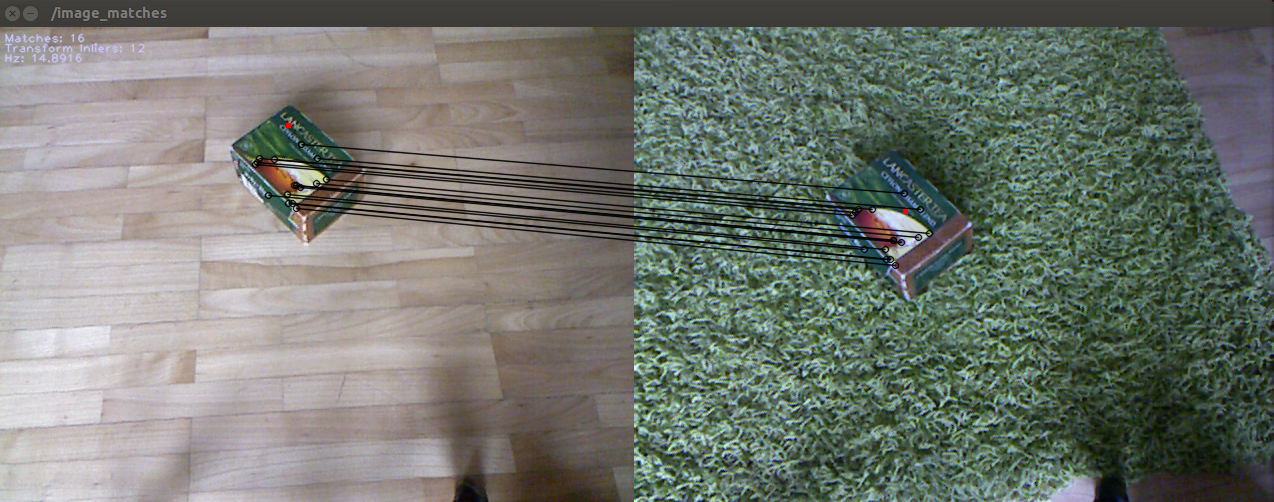
\includegraphics[width=0.7\columnwidth]{figures/brief-no-rotation.png}\\
%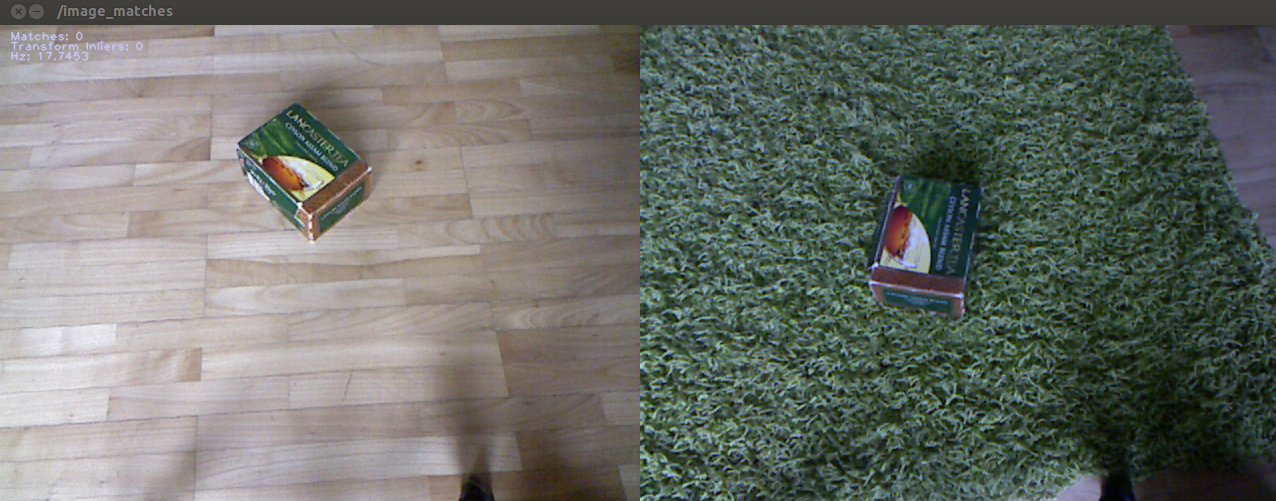
\includegraphics[width=0.7\columnwidth]{figures/brief-rotation.png}\\
%    \end{tabular}


%\caption{Comparison of two pairs of images using FAST detector and BRIEF descriptor. The upper image shows the object in the original pose whereas the lower shows the rotated object. It can be noticed that number of feature matches significantly decreases if the object is rotated. }
%\label{fig:brief-features}
%\end{figure}


\subsection{View-point Variance}

In order to show the problem of view-point variance of the feature descriptors we compared two live images of the same object - one in the same pose as it is in the database and the other one when the object is rotated around Z (upright) axis. We tested those pairs with two different detectors and descriptors to ensure that the problem is not connected to a particular detector-descriptor pair. The results are depicted in Figure \ref{fig:sift-features} and \ref{fig:freak-features}.% and brief-features}.

Looking at Figure \ref{fig:sift-features} and \ref{fig:freak-features} it is noticeable that the number of matches significantly decreases when the object is rotated. Even with the most rotationally and view-point invariant feature detector-descriptor pair - SIFT (see Figure \ref{fig:sift-features}) - drop of the features equals 35$\%$.



\section{Approach}

Following our idea to leverage robot's capabilities in order to improve its perception skills, we employ interaction with object as a mean that is likely to partially solve one of the above mentioned challenges. In our approach we use the rotational movement of the object in order to eliminate the influence of view-point variance of features. Our goal is to keep rotating the object until we put it in the configuration that the system was trained on, thus, we are more likely to find more feature matches and successfully recognize the object. We observed that translational movements do not influence the efficiency of the recognition system. However, it is crucial to translate the object as little as possible while rotating it so that it does not move out of the area that is visible to the robot. In the next section we show our method of efficient rotation of the object without significant energy loss resulting in translational movement.

\begin{figure}
\centering 

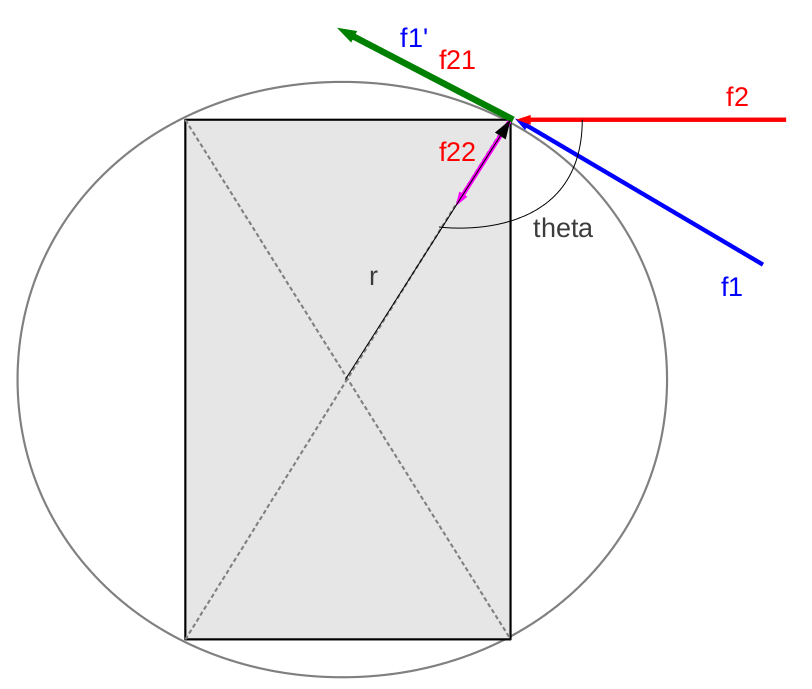
\includegraphics[width=0.5\columnwidth]{figures/rectangle-angle.png}\\


\caption{Object under the influence of two forces. f1 shows the tangential push that will result it in only rotational movement, hence in the force - f1\' tangential to a circle exscribed on the object. f2 shows the proposed pushing strategy - perpendicular to the longer egde. This push results in two forces - f21 tangential coefficient responsible for rotation and f22 - translational coefficient. In this case object will not only rotate but also translate in the direction of f22 force.  }
\label{fig:angles-rectangle}
\end{figure}


\begin{figure}
\centering
 

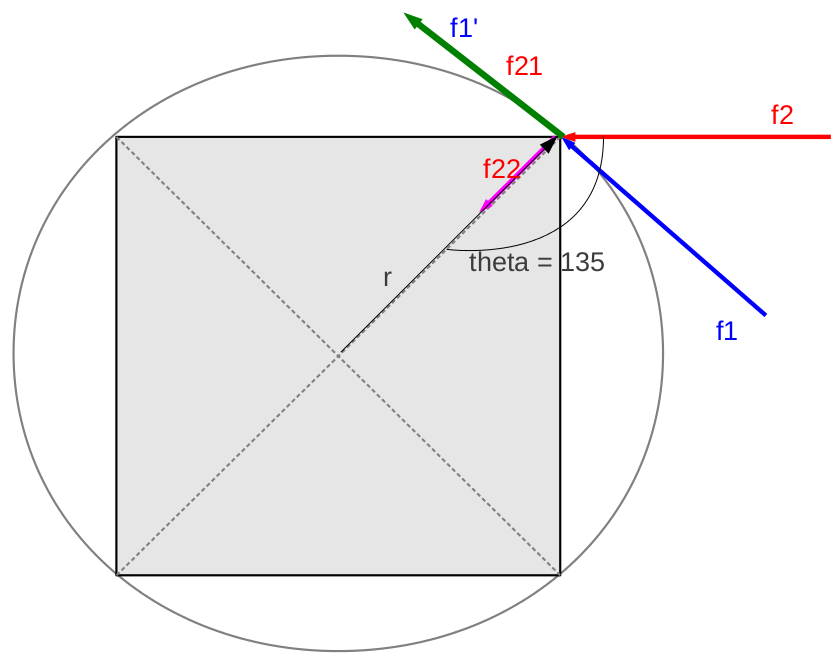
\includegraphics[width=0.5\columnwidth]{figures/square-angle.png}


\caption{Extreme example of energy loss of the proposed pushing strategy on the squared object. $\theta$ is in this case maximal and equals $135 ^\circ$. It results in a energy loss of 29\%.  }
\label{fig:angles-square}
\end{figure}

\begin{figure}
\centering 

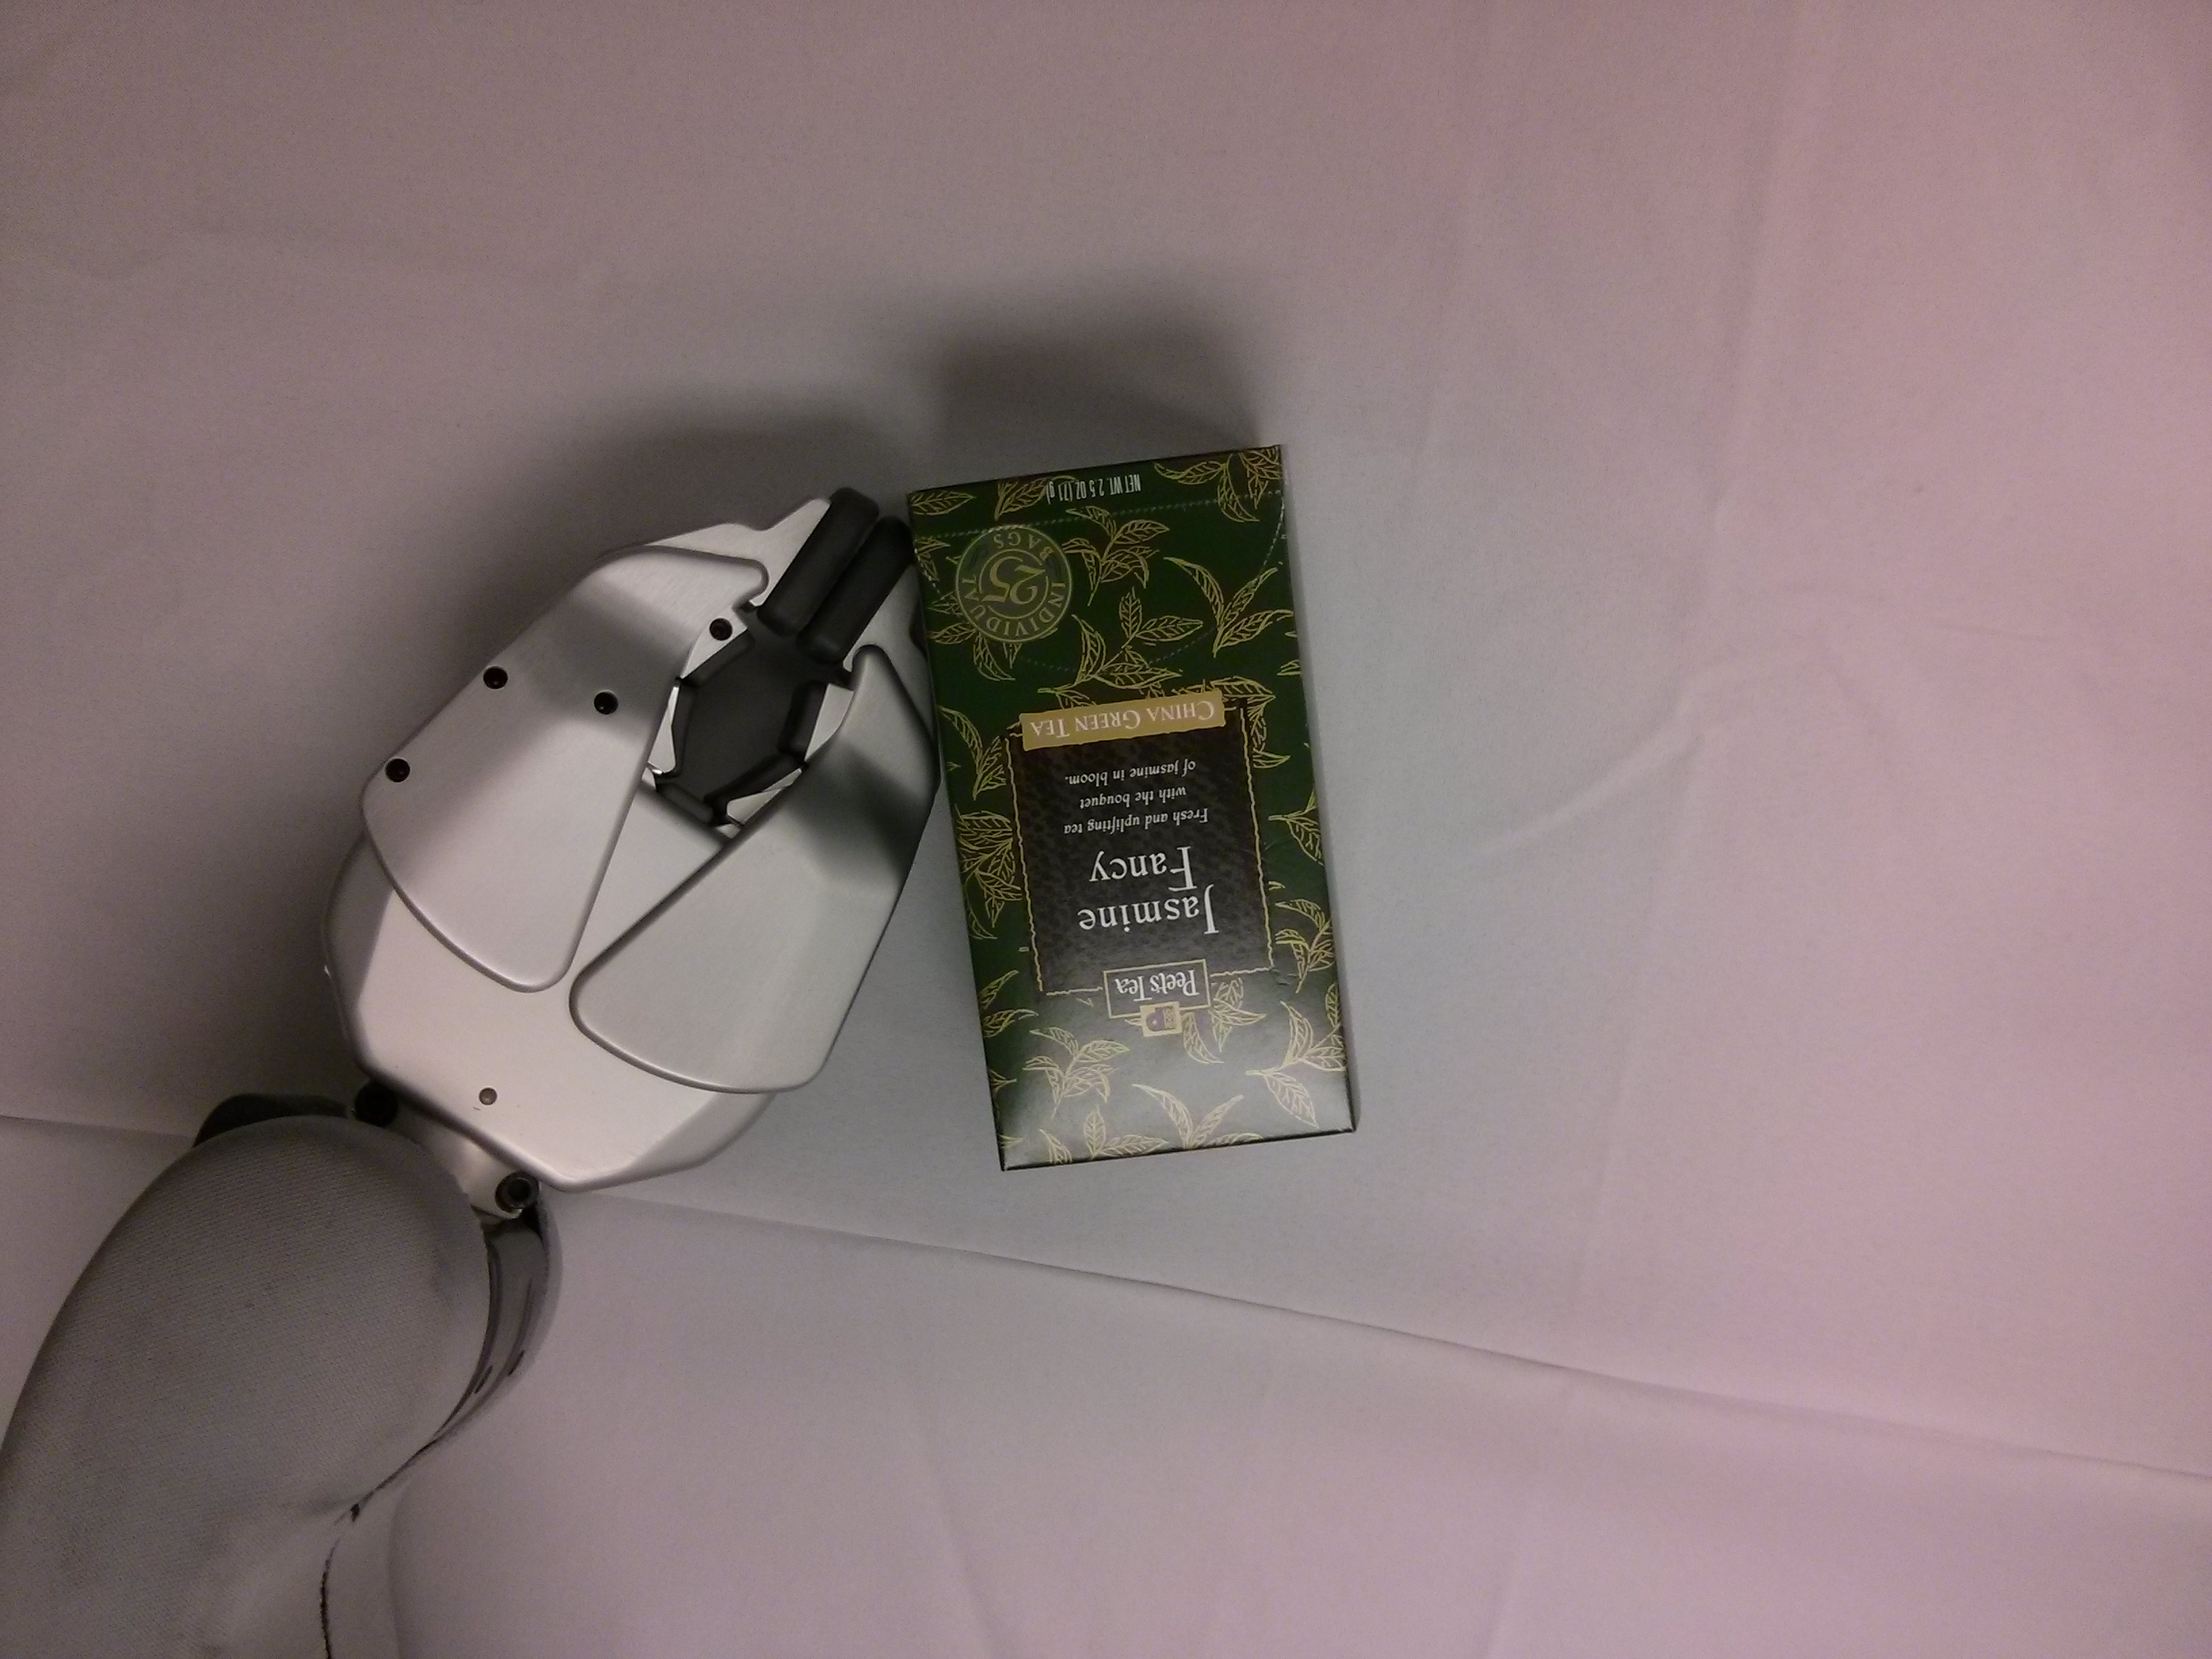
\includegraphics[width=0.4\columnwidth]{figures/peets-tangential.jpg}\\
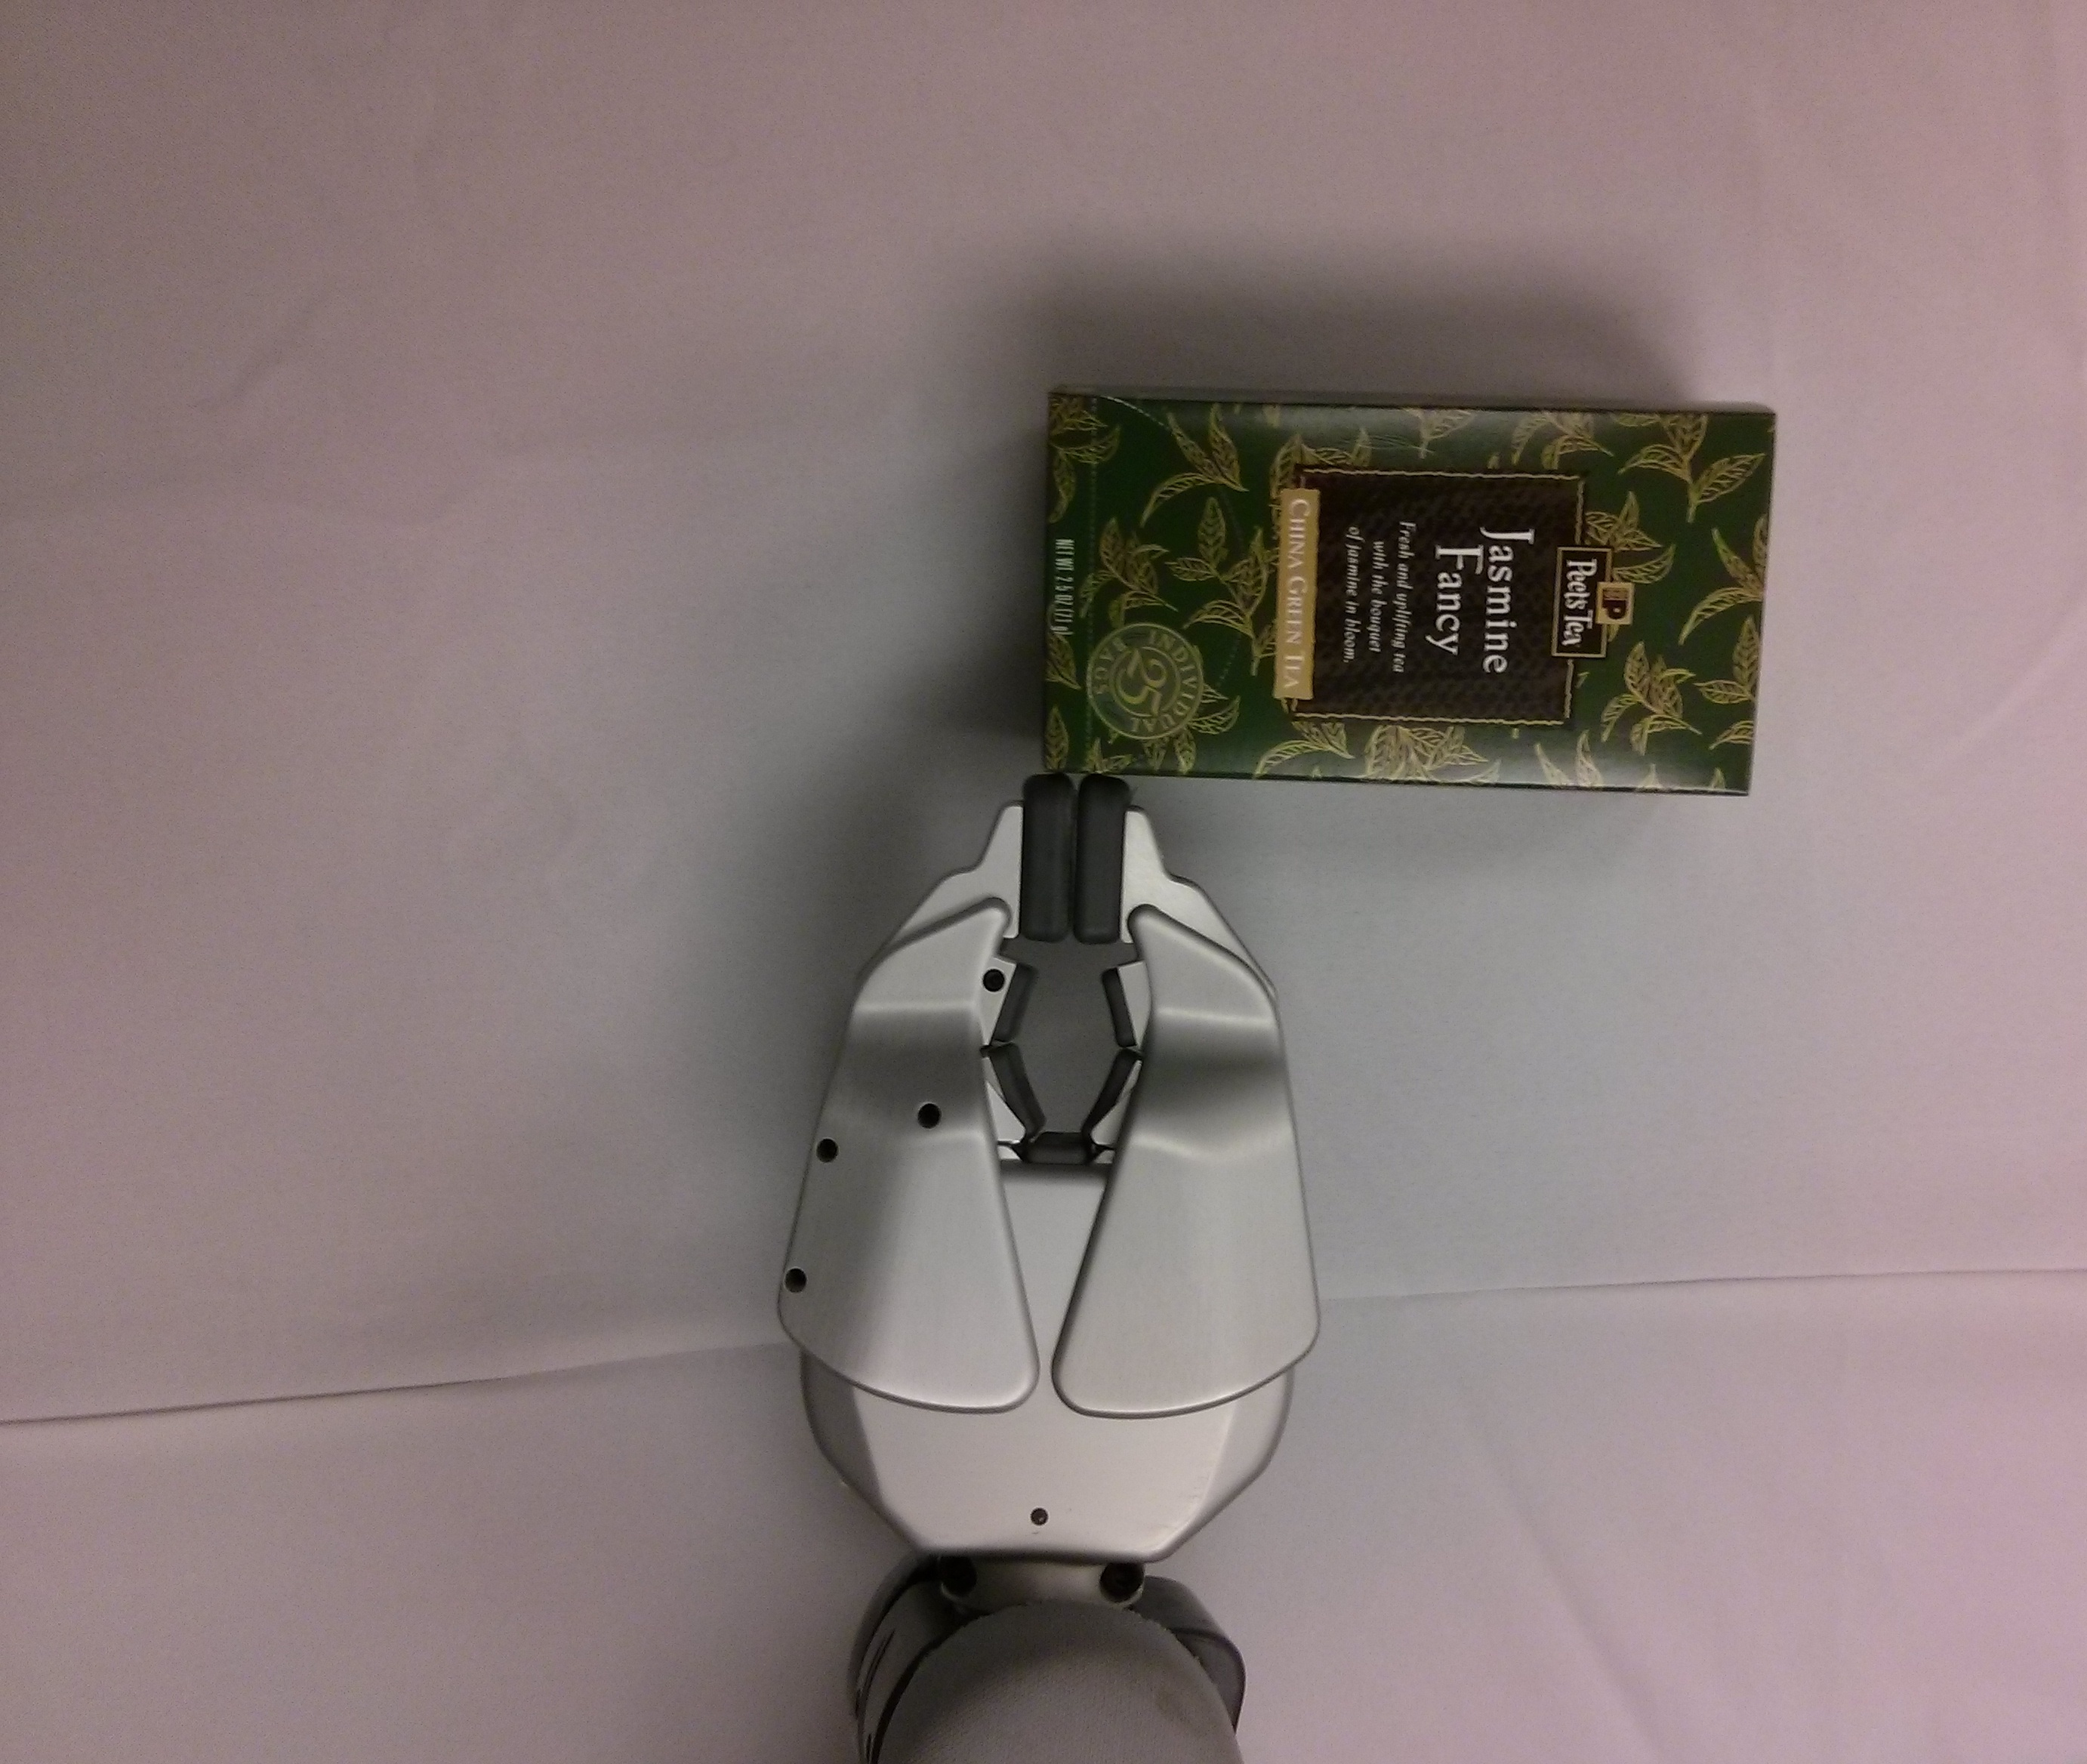
\includegraphics[width=0.4\columnwidth]{figures/peets-perpendicular.jpg}\\


\caption{Upper row - example of tangential push. Lower row - example of perpendicular push.}
\label{fig:tangential-example}
\end{figure}


\subsection{Rotation of Objects}
In order for a robot to rotate an object efficiently, meaning that the push results in only rotational kinematic energy, it is required to maximize the torque acting on the object. As shown in Equation \ref{eq:max-torque} the maximum torque($M$) can be obtained with the biggest radius ($r$ component) that the force($F$) is acting on and with $sin(\theta) = 1$. Where $\theta$ is the angle between the force and the radius.

\begin{equation}
M =  F \times r = F*r*sin(\theta)\\
\label{eq:max-torque}
\end{equation}

Maximizing $r$ component results in the point that is the furthest from the center of mass of the object. Since we assume uniform distribution of mass, the center of mass of the object is in its geometrical center. Hence the best push point to rotate the box-like object is at the corner which is the furthest point from the center of the rectangle.

In order to fulfil the second constraint: $sin(\theta) = 1 \to \theta = 90 ^\circ$, a robot needs to perform a tangential push. The resulting force f1 showing this case on a box-like object is depicted in Figure \ref{fig:angles-rectangle}. However, due to geometrical constraints of the robot's gripper it is difficult to execute tangential push. The upper row of Figure \ref{fig:tangential-example} shows the box-like object with the robot's gripper in the pose for the tangential push. It can be noticed that due to the size of the gripper the actual contact point between the gripper and the object is not at the corner. The other problem that occurs in this kind of push is that the gripper is likely to slip off the object while pushing.

Because of the above mentioned reasons we propose a push perpendicular to the longer edge of the object. This push is easy to execute with the robot's gripper while still being able to result in rotational movement of the object. The lower row of Figure \ref{fig:tangential-example} shows the resulting robot's gripper position relative to the object. However, in this case the push is not optimal in the sense that $\theta$ is not $90 ^\circ$. In order to evaluate how much energy loss to translational movement is obtained we theoretically analyzed the above described scenario. Figure \ref{fig:angles-square} shows a square object where $\theta$ is maximal thus the least optimal for the function $sin(\theta)$. By simple geometric analysis one can show that $\theta =135 ^\circ$ which results in $sin(\theta) = 0.71$. The result of this theoretical experiment shows that in the worst case scenario (squared object produces the worst possible $\theta$) one loses 29\% of the resulting kinematic energy on translational movement. Given the robot's configuration and the size of its gripper the loss is acceptable as it still results in mostly rotational movement of the object. 

Having developed the method to rotate the object, we want to investigate the improvement of the actual object recognition system that is done by inducing the motion of an object into the scene. We claim that rotating the object significantly improves the chances of the object being recognized correctly and it makes the feature-based object recognition system more computationally efficient.

\subsection{Object Recognition System}

In this section we show the software architecture that lies behind the object recognition system we created. The system was divided into 5 ROS packages with different responsibilities:
\begin{itemize}
\item Cloud Saver - a ROS package responsible for saving the live image from the Kinect sensor in the database. A user is given a simple user interface where they can see the live image from the Kinect. It has options to save the current image together with the associated point cloud. Using this package we can create the library of images that will be later used as the database of objects that a robot is able to recognize.
\item PCL I/O - a helping package that is mainly responsible for reading, writing and loading different PCL structures. It is heavily used especially in the Cloud Saver package.
\item Object Library - the main purpose of this ROS package is to generate the data for different images that were taken with Cloud Saver. It wraps all the data into an object data structure which contains the image and the name of the object and is easily extensible to contain more information in the future.
\item Features - a class in a ROS package that has all the functionality to extract, describe and match different computer vision features. The features that currently implemented in this class hold OpenCV implementations of various detector-descriptor pairs such as: SIFT, SURF, FREAK, FAST, BRIEF, ORB and STAR. It is extensively used throughout the matching phase of the system.
\item Object Matcher - the main ROS package that matches all the previous elements together. It loads all the data prepared by the Object Library package which forms a library of objects that are used as models in the systems. After all the objects are loaded, it calls Features class to compute matches between live images and images in the database. At the end it outputs the score that indicates if the object was recognized and which object it is.
\end{itemize}


The packages described above form an object recognition system that enables a user to easily acquire data from a Kinect device, create a library of objects to recognize, and finally, extract, describe and match various computer vision features that will lead to a final result - a recognized object.




\section{Results}

\begin{figure}
%\centering 

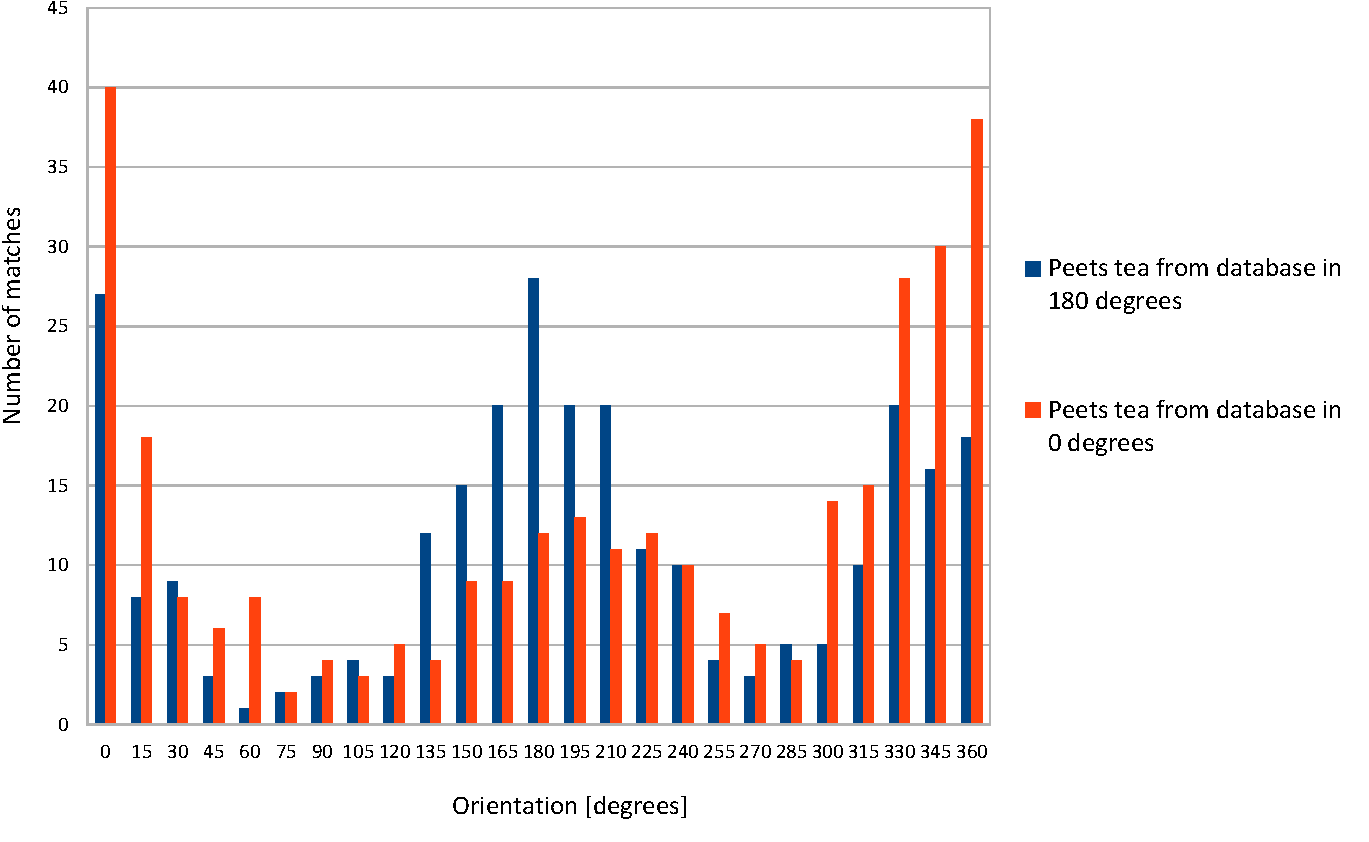
\includegraphics[width=1.3\columnwidth]{figures/print2.pdf}\\


\caption{Chart showing matching results between two images of the peets tea from the database and the live image of the peets tea. Peets tea was moved 360$^\circ$ during the matching process. One image from the database shows the peets tea in the orientation 0$^\circ$ and the second one in the orientation 180$^\circ$. One can notice that the peaks of the number of matches are in 0$^\circ$, 180$^\circ$ and 360$^\circ$.}
\label{fig:recognition-results}
\end{figure}
%Experiments showing time with multiple templates
%Graph of different numbers of matches in relation to degrees
Since we already introduced the basic idea, the algorithms and the software used in this system, in this section we show how the system is evaluated on the real objects.

The testing set-up of the system consists of an object that is in front of the Kinect. During the experiment the object is rotated 360$^\circ$ according to our movement strategy described in the previous section. The live image is compared to all the images from the database. Database consists of two images per object. In the second image the object is rotated 180$^\circ$ with respect to its previous position (represented in the first image in the database). During this process the number of matches is constantly saved to a file. The system is trained on two objects: Peets tea and Lipton tea and evaluated on the former one. The recognition procedure is repeated three times and the results were averaged in order to reduce noise in our measurements. 

Figure \ref{fig:recognition-results} shows the averaged number of matches relative to the orientation of the object. The vertical axis shows the number of matches between the live image and the image described by the respective color (see legend in Figure \ref{fig:recognition-results}). Generally, it can be seen that there are certain configurations where the number of matches is significantly greater. These relate to the configurations close to the pose of the object that appear in the image from the database. It shows that rotating the object in uninformative manner can significantly improve its recognition. 

One can also notice that both plots in Figure \ref{fig:recognition-results} have smaller picks at the position which is 180$^\circ$ from the original pose of the object in the database. This happens due to the symmetry of some of the features on the object used in that experiment. Those features appear similar if they are rotated by 180$^\circ$, hence we obtain additional matches if the object is rotated by 180$^\circ$ with respect to the pose the algorithm was trained on.

\begin{figure}
\centering 

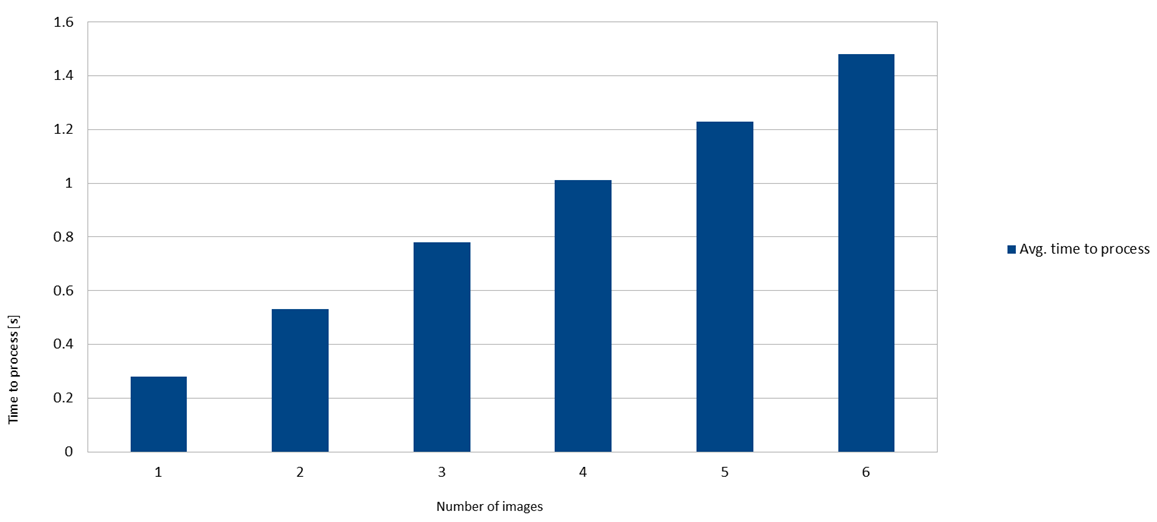
\includegraphics[width=1.2\columnwidth]{figures/thesis-time.png}\\


\caption{The processing time of the object recognition algorithm with different number of images in the database.}
\label{fig:recognition-time}
\end{figure}

Approximate time for the system to process the data with two 640-480 resolution images during one iteration equalled $0.53 sec$. In one iteration we generate the matches between the live image and all the images from the database. During one iteration there was approximately 100 features found in one image. In Figure \ref{fig:recognition-time} it can be noticed that the time of iteration linearly scales to the number of images. Hence, the computational cost to recognize an object is scaled by the number of images per object in the database. By decreasing the number of images per object, we can radically decrease the computational cost of the object recognition algorithm. Thus, inducing motion into the scene and reducing the size of the database has a significant impact on the system performance.





\section{Conclusion}
We have presented an initial implementation of the system that is able to recognize objects based on feature matching algorithm. We have proven that inducing motion into the scene significantly improves chances of the object being recognized correctly. In addition to that we showed that interaction with the scene reduces the size of the database which has a significant influence on the speed of the system.  
